\section{A mathematical treatment of worlds and their transformations}\label{sec:Mathematical framework for an agent in an environment}

\newthought{We want our} framework to be as general as possible, so we consider worlds as consisting a set of world states, which are distinguishable in some way\footnote{We are building up to using our framework to consider the transformation structure of the world from the perspective of an agent. So when we say \emph{distinguishable in some way} we mean that there is some way for our agent to distinguish between the states.}, and a set of transformations between those world states; these transformation describe how the current state of the world can be changed to other states (\textit{i.e.} the \emph{dynamics of the world}).

We will also make a few simplifications to the worlds we consider:
\paragraph{Deterministic worlds.}
In a deterministic world, every change in the current world state has a single guaranteed effect.
A world that is not deterministic is called \emph{stochastic}; in a stochastic world, the same change to the current world state could produce different results.
We will initially consider deterministic worlds.

\paragraph{Fully observable worlds.}
If complete knowledge of the current world state for every possible current world state is known\footnote{This does not mean knowledge of the transformations between world states. Also, it does not mean knowledge of every world state, but knowledge of the current world state, no matter which world state is the current one}, then the world is called \emph{fully observable}; if not then the world is called \emph{partially observable}.
Partially observable worlds are common in many real-world scenarios, however, we will initially consider fully observable worlds.
\footnote{Move this section to agents section? "When an agent sensor is capable to sense or access the complete state of an agent at each point in time, it is said to be a fully observable environment else it is partially observable."}

We begin with fully observable worlds because:
\begin{itemize}
    \item their treatment is simpler than partially observable worlds, and
    \item the representation of an agent of a partially observable world should ideally be the same as the representation of the agent in the same world but fully observable; therefore, if we identify structures present in an agent's representation of fully observable worlds then we are also identifying structures that should be present in the agent's representation of the same world but partially observable without having to consider the complications of partial observability\footnote{???}.
\end{itemize}

\paragraph{Discrete worlds.}
In a \emph{discrete} world, the number of states and the number of transformations between states are countable.
A world that is not discrete is called \emph{continuous}.
For simplicity, we only consider discrete worlds.
However, we argue that it is actually more natural to consider discrete worlds.
Consider an agent with $n$ sensors $\theta_{n}$ that can interact with a world $\mathscr{W}$ using continuous actions $A$ to produce a sensor observation: $\theta_{i}(w) = o_{i}$ where $i \in \{1, ..., n\}$ and $w \in W$.
We hypothesise that there will be actions $da \in A$ that cause changes in the world state that are so small that the agent's sensors will not perceive the change (\textit{i.e.}, $\theta_{i}(da * w) = o_i$).
Therefore, there will be discrete jumps between perceptible states of the world in the agent's representation.

\newthought{Before we formally} define our generalised worlds, we need to talk about how transformations are made up of smaller transformations.
We say that the smallest transformations\footnote{Note that, in the same way as for distinguishable world states, when we use our framework to describe the representation of an agent, these smallest transformations will be the smallest transformations detectable by the agent.} in our world are called \emph{minimum transformations}.
We denote a transformation as a minimum world state transformation or a set of transformations as a set of minimum transformations using a $\hat{ }$.
Soon we will combine these minimum transformations to give us all the transformations for the world, but first we need to establish some properties of minimum transformations.

Let the set of minimum world state transformations be $\hat{D}$ and the set of world states be $W$.
We define two maps $\hat{s},\hat{t}: \hat{D} \to W$; $\hat{s}$ is called the \emph{source map} and $\hat{t}$ is called the \emph{target map}.
For any minimum world state transformation $\hat{d} \in \hat{D}$ from a world state $w_{1} \in W$ to a world state $w_{2} \in W$, $\hat{s}(\hat{d}) = w_{1}$ and $\hat{t}(\hat{d}) = w_{2}$.

\newthought{We can now} formally define our generalised worlds as a directed multigraph.
A \emph{world} $\mathscr{W}$ is a directed multigraph $\mathscr{W} = (W, \hat{D}, \hat{s}, \hat{t})$ where $W$ is a set of \emph{world states}, $\hat{D}$ is a set of \emph{minimum world state transformations}, and $\hat{s},\hat{t}: \hat{D} \to W$ are the source and target maps.

\newthought{We are interested} in the all the transformations of our world $\mathscr{W}$, not just the minimum transformations.
We let the set of all paths in $\mathscr{W}$ be called the set of all transformations and denote it by $D$; we call the elements of $D$ transformations\footnote{Minimum transformations are also transformations.}.
A transformation $d \in D$ is a sequence of minimum world state transformations $d = \hat{d}_{n} \hat{\circ} \hat{d}_{n-1} \hat{\circ} ... \hat{\circ} \hat{d}_{1}$, where $\hat{\circ}: \hat{D} \times \hat{D} \to D$ is a composition operator\footnote{This operator is the operator of concatenation of paths.} that is defined if $\hat{t}(\hat{d}_{i}) = \hat{s}(\hat{d}_{i+1})$ for $i = 1, ..., n-1$.
The composition operator $\hat{\circ}$ is associative\footnote{If an operator $\cdot$ is \emph{associative}, it means that when we perform the operation $\cdot$ on three or more elements, the way in which the elements are grouped does not affect the outcome; this is commonly defined by the condition $a \cdot (b \cdot c) = (a \cdot b) \cdot c$.} by the definition of concatenation of paths.
We have constructed our transformations this way because it means that each transformation in $D$ can be represented as a unique composition of minimum transformations. 
The \emph{length} of a transformation is the number of minimum transformations in its unique composition of minimum transformations\footnote{This means minimum transformations have a length of one.}.

\paragraph{Trivial transformations.}
For each world state $w \in W$ there is an element in $\hat{D}$ that represents a path with no transformations that starts and ends at $w$ (\textit{i.e.}, $\hat{s}(1_{w}) = \hat{t}(1_{w}) = w$); this element is denoted by $1_{w}$.
These transformations are called \emph{trivial transformations}\footnote{Trivial transformations essentially represent nothing happening; we will hear more about this when we look at the actions of agents.}.
Trivial transformations serve as a neutral element in path concatenation; this means trivial transformations do not alter other paths when they are composed with them\footnote{This property of trivial transformations is part of the definition of path concatenation and is analogous to the identity element in algebraic structures.}: for any $\hat{d} \in \hat{D}$, $d \hat{\circ} 1_{\hat{s}(d)} = d$ and $1_{\hat{t}(d)} \hat{\circ} d = d$ \footnote{Due to this aspect of the definition of trivial transformations, transformation sequences involving trivial transformations are not distinct elements in $D$ (except for the sequences of containing only a single trivial transformation).
For example, $\hat{d} \hat{\circ} 1_{\hat{s}(\hat{d})}$ is the same element in $D$ as $\hat{d}$.}.
Due to this behaviour, trivial transformations are said to have a length of zero.

\paragraph{From $\hat{D}$ to $D$.}
We extend the minimum transformation source map $\hat{s}$ and target map $\hat{t}$ of $\hat{D}$ to a source map $s: D \to W$ and a target map $t: D \to W$ of $D$.
$s$ is defined such that for any $d \in D$ with $d = \hat{d}_{n} \hat{\circ} \hat{d}_{n-1} \hat{\circ} ... \hat{\circ} \hat{d}_{1}$, $s(d) = \hat{s}(\hat{d}_{1})$.
$t$ is defined such that for any $d \in D$ with $d = \hat{d}_{n} \hat{\circ} \hat{d}_{n-1} \hat{\circ} ... \hat{\circ} \hat{d}_{1}$, $t(d) = \hat{t}(\hat{d}_{n})$.

We also extend the minimum transformation composition operator $\hat{\circ}: \hat{D} \times \hat{D} \to D$ to a composition operator $\circ: D \times D \to D$ that is defined for $d' \circ d$ if $t(d) = s(d')$.
For any $d, d' \in D$ with $d = \hat{d}_{n} \hat{\circ} \hat{d}_{n-1} \hat{\circ} ... \hat{\circ} \hat{d}_{1}$ and $d' = \hat{d'}_{n} \hat{\circ} \hat{d'}_{n-1} \hat{\circ} ... \hat{\circ} \hat{d'}_{1}$, $d' \circ d = d''$ where $d'' \in D$ is defined, $d'' = \hat{d'}_{n} \hat{\circ} \hat{d'}_{n-1} \hat{\circ} ... \hat{\circ} \hat{d'}_{1} \hat{\circ} \hat{d}_{n} \hat{\circ} \hat{d}_{n-1} \hat{\circ} ... \hat{\circ} \hat{d}_{1}$.
$\circ$ is associative following from the associativity of $\hat{\circ}$.

Since the extended source map $s$, target map $t$, and composition operator $\circ$ encompass the minimum transformation source map $\hat{s}$, target map $\hat{t}$, and composition operator $\hat{\circ}$, we will use the extended $s$, $t$, and $\circ$ in the remainder of this work.
Additionally, it is easy to see that the neutral element properties of trivial transformations hold for any transformation in $D$\footnote{For any $d \in D$, $d \circ 1_{s(d)} = d$ and $1_{t(d)} \circ d = d$.}.
For a transformation $d \in D$ with $s(d) = w$ and $t(d) = w'$, we will often denote such a $d$ by $d: w \to w'$.




\newthought{We can visually} represent the structure of our directed multigraphs using \emph{world diagrams} consisting of a dots for the world states and arrows for the transformations.
These diagrams can make it easier to understand the structure and properties of worlds.


\autocite{barr1990category}\footnote{test 
\autocite{barr1990category}
}

Since our set $D$ is can be very large\footnote{
If we have transformations $d: s(d) \to t(d)$ and $d': s(d) \to t(d)$, then we can construct sequences like $d' \circ d$, $d' \circ d \circ d' \circ d$ etc..., which means $D$ has an infinite number of elements:
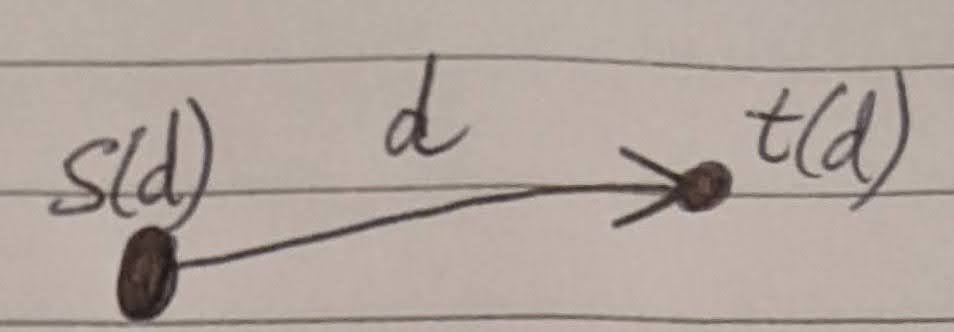
\includegraphics[width=0.5\linewidth]{2MathematicalFramework/InitialFramework/Images/transformation.jpg}


% \begin{figure}
%     \centering
%     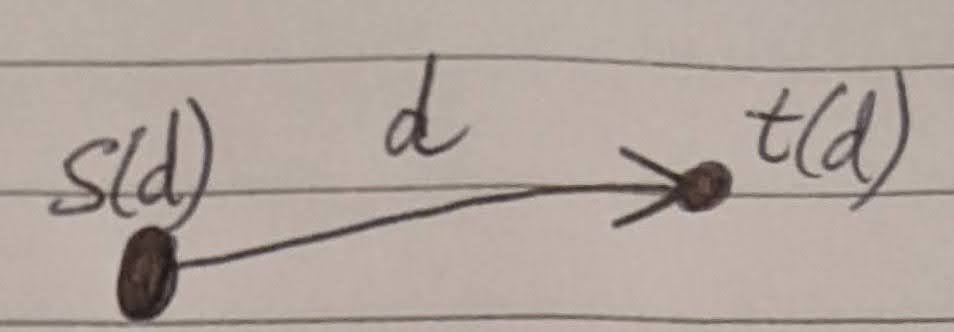
\includegraphics[width=0.5\linewidth]{2MathematicalFramework/InitialFramework/Images/transformation.jpg}
%     \caption{Caption}
%     % \label{fig:transformation}
% \end{figure}
}, we do not show all the transformations in $D$ in our world diagrams unless explicitly stated.


\begin{figure}
    \centering
    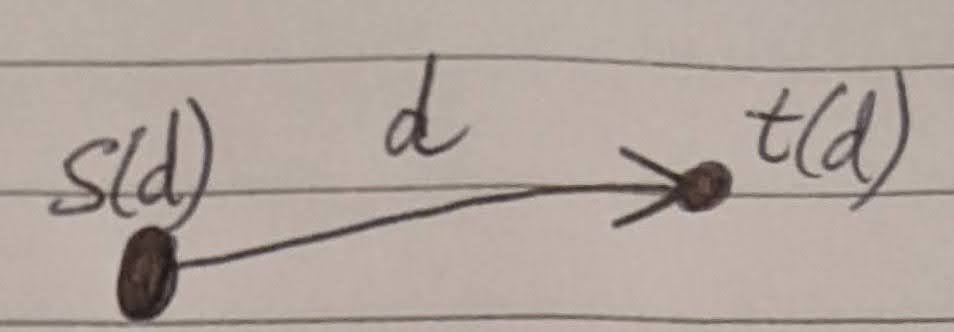
\includegraphics[width=0.5\linewidth]{2MathematicalFramework/InitialFramework/Images/transformation.jpg}
    \caption{Caption}
    \label{fig:transformation}
\end{figure}

\begin{figure}
    \centering
    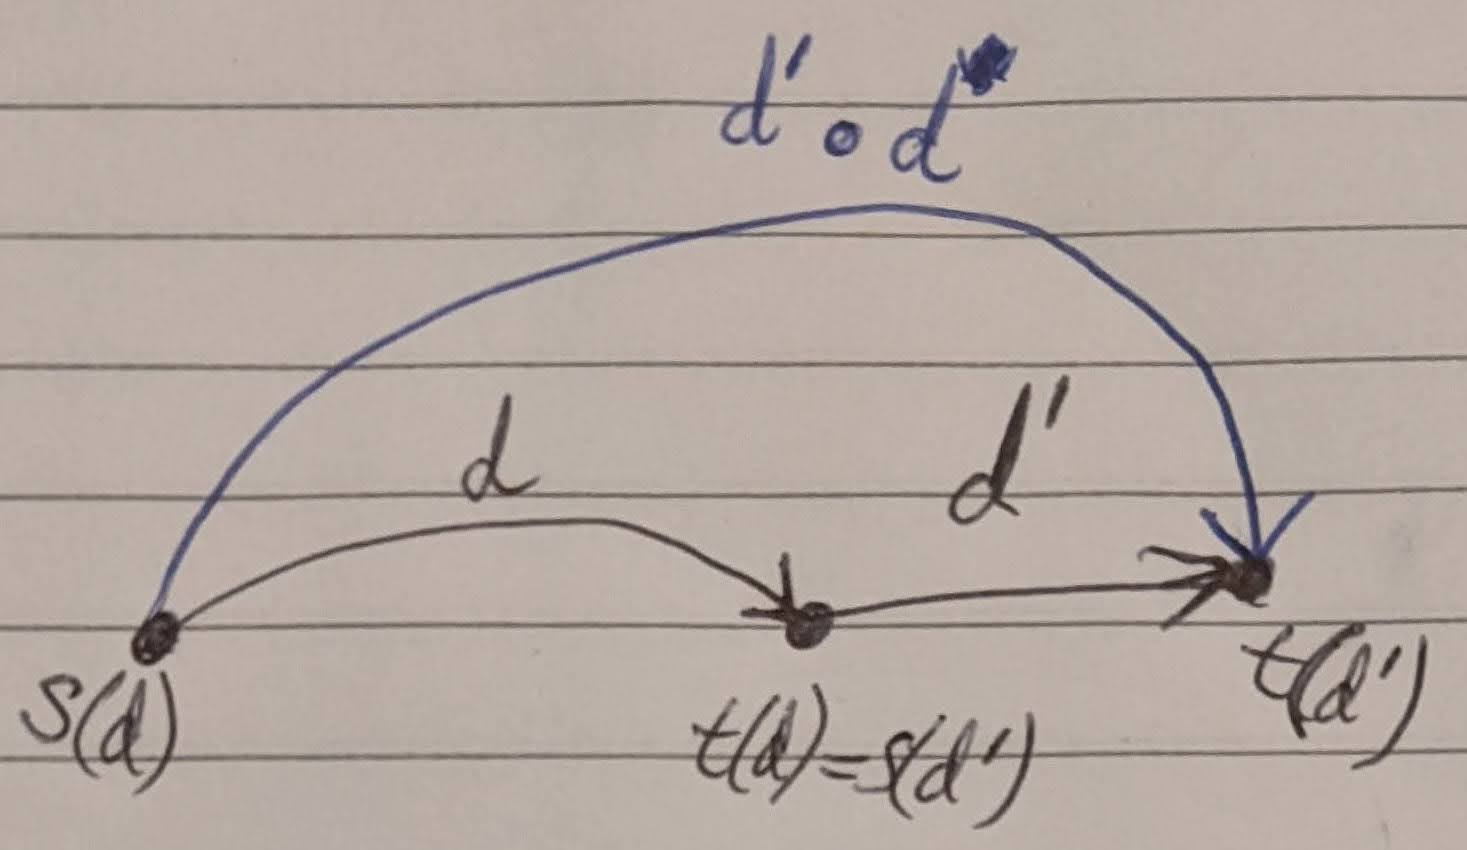
\includegraphics[width=0.5\linewidth]{2MathematicalFramework/InitialFramework/Images/transformation_composition.jpg}
    \caption{Caption}
    \label{fig:transformation_composition}
\end{figure}

\begin{figure}
    \centering
    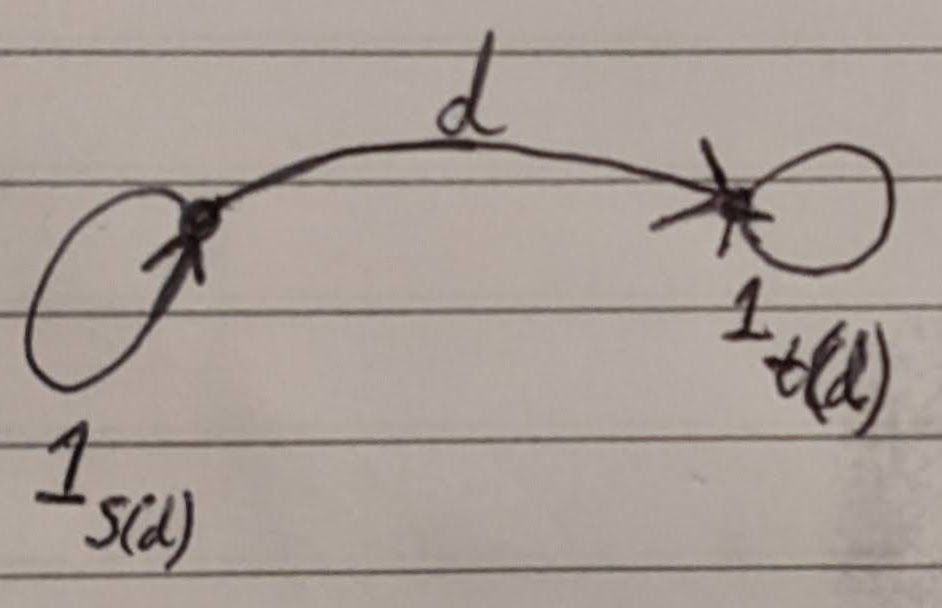
\includegraphics[width=0.5\linewidth]{2MathematicalFramework/InitialFramework/Images/trivial_transformations_example_all_transformations.jpg}
    \caption{Caption}
    \label{fig:trivial_transformations_example_all_transformations}
\end{figure}

\begin{figure}
    \centering
    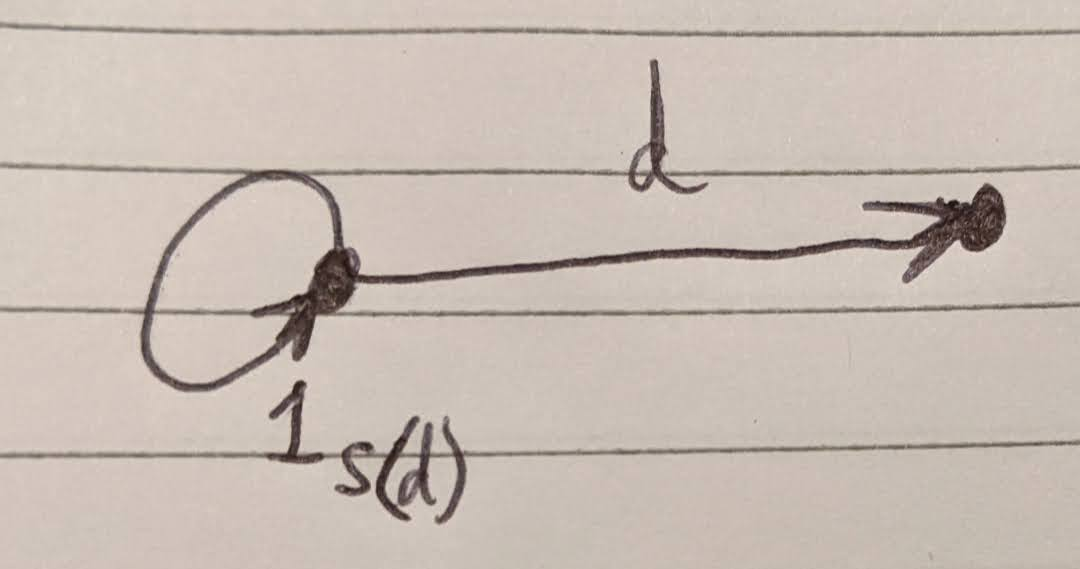
\includegraphics[width=0.5\linewidth]{2MathematicalFramework/InitialFramework/Images/right_trivial_transformation.jpg}
    \caption{Caption}
    \label{fig:right_trivial_transformation}
\end{figure}

\begin{figure}
    \centering
    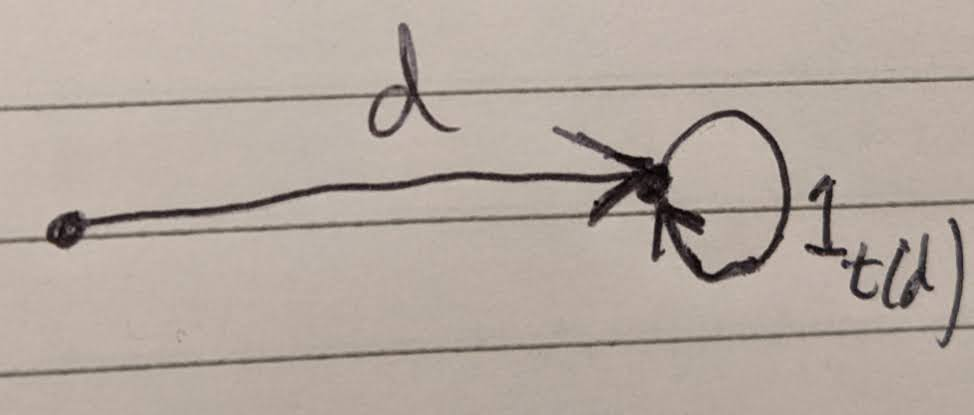
\includegraphics[width=0.5\linewidth]{2MathematicalFramework/InitialFramework/Images/left_trivial_transformation.jpg}
    \caption{Caption}
    \label{fig:left_trivial_transformation}
\end{figure}



\noindent\rule{\textwidth}{1mm}

% \begin{marginfigure}
%     \centering
%     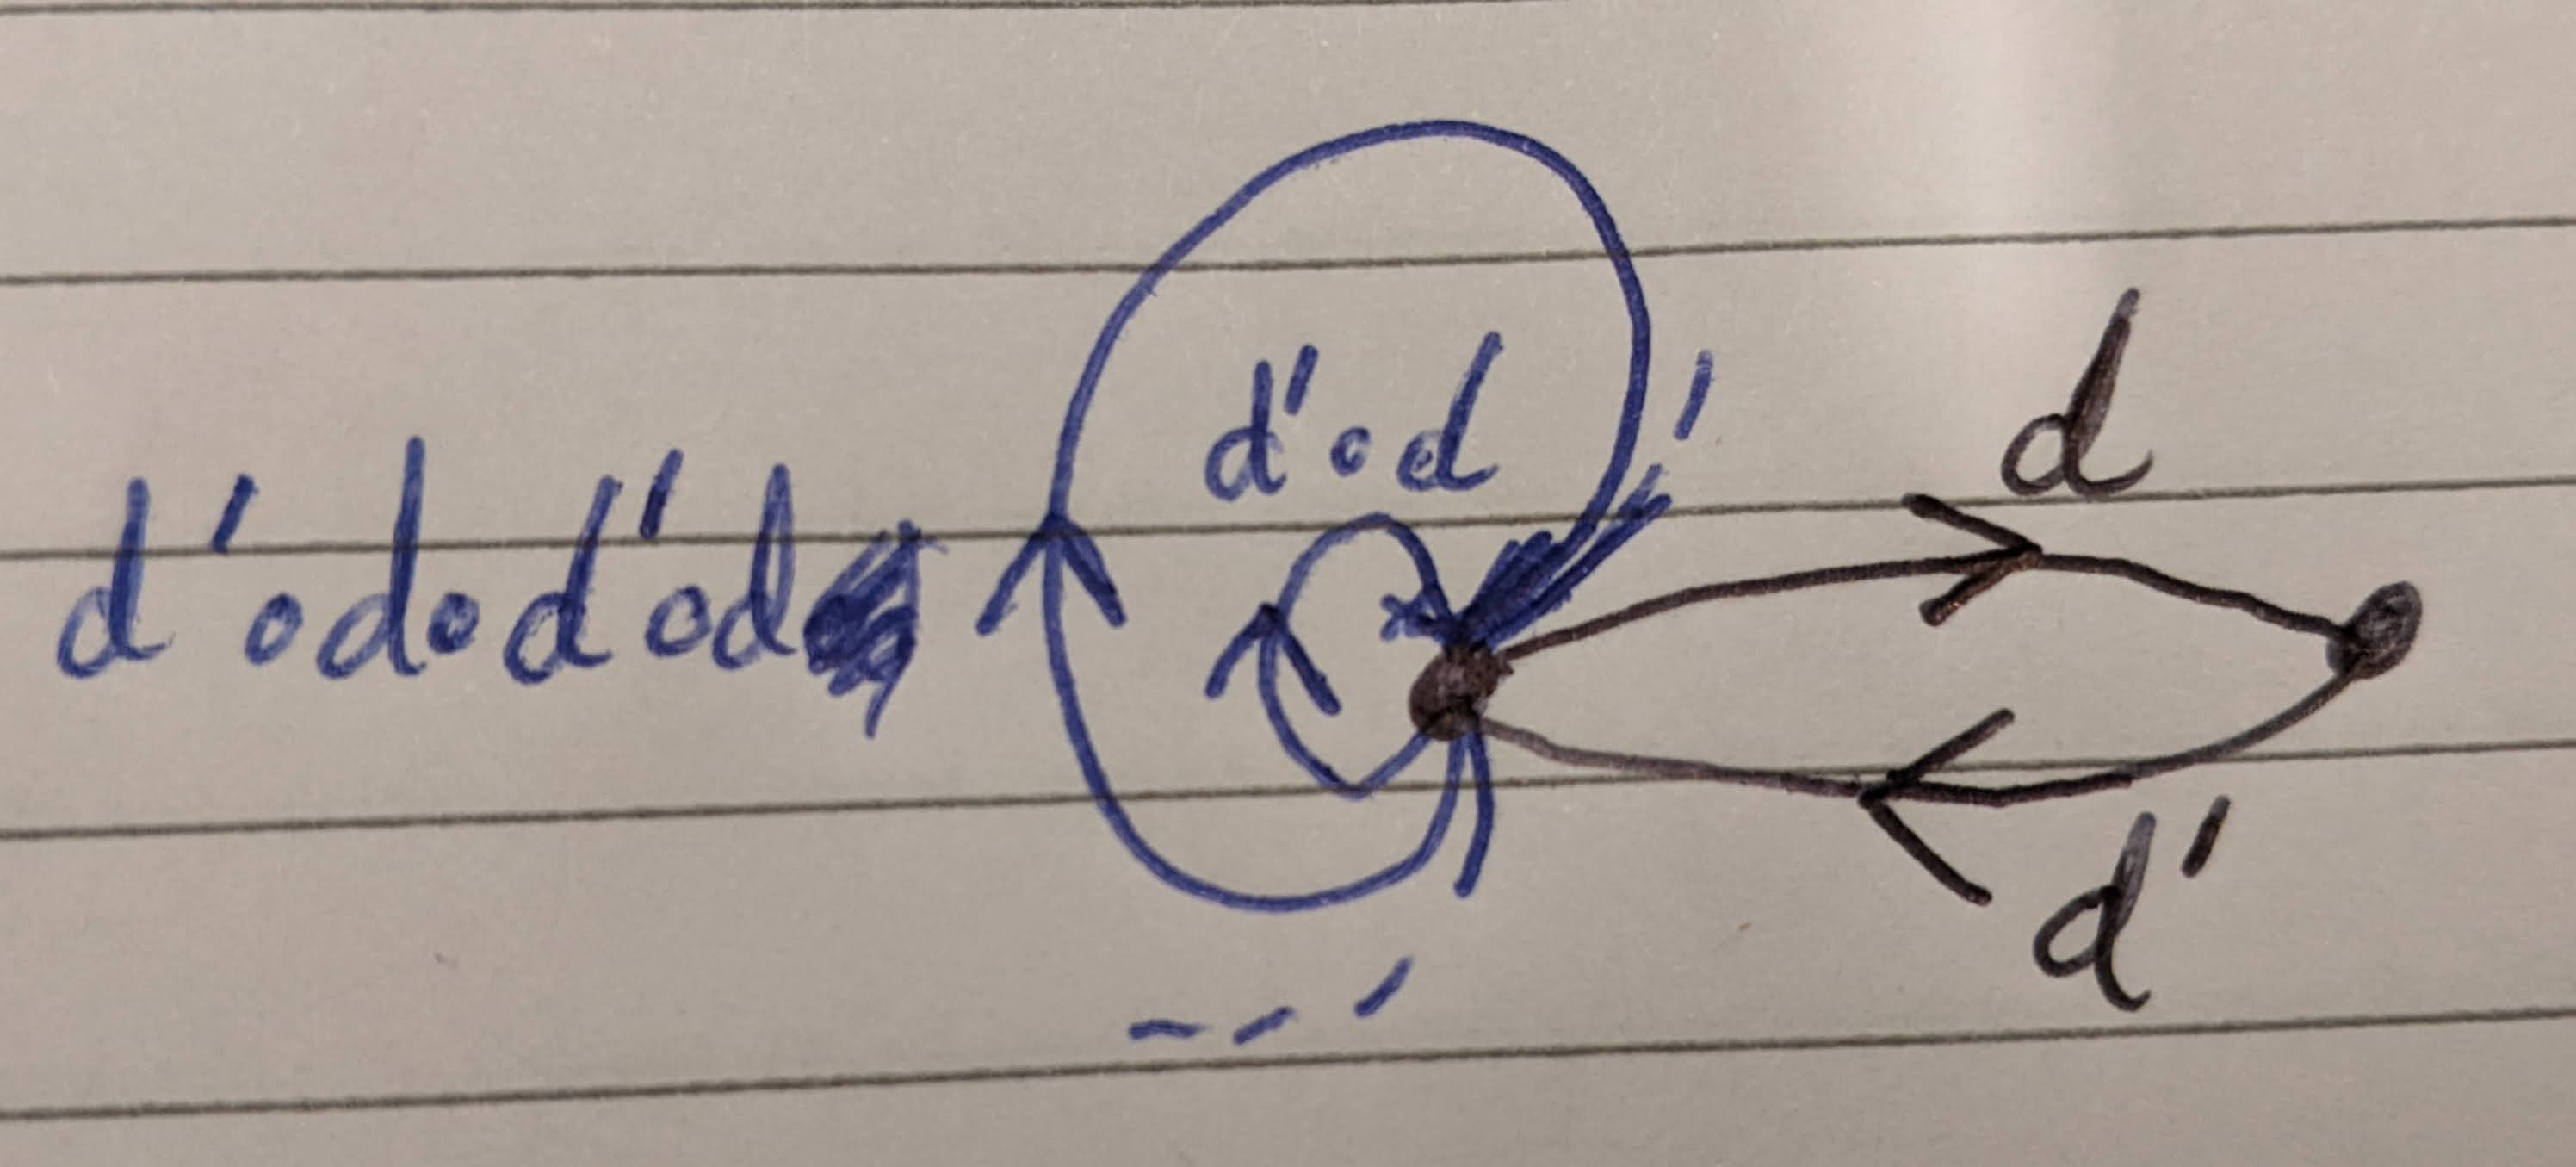
\includegraphics[width=0.5\linewidth]{2MathematicalFramework/InitialFramework/Images/D_commonly_large.jpg}
%     \caption{Caption}
%     \label{fig:enter-label}
% \end{marginfigure}

\textbf{Diagrams:}
\begin{enumerate}
    \item Transformation.
    \item Composition of transformations.
    \item Trivial transformation, both rules.
    \item No unique element in $D$ for sequence with trivial transformations.
\end{enumerate}

\begin{itemize}
    \item Figure out how to put a figure in a side note.
    \item Write figure captions.

    \item Mention: we can have more than one minimum transformation between two states. Why we allow this becomes clear when we introduce the idea of agent actions.
    \item Mention: positioning of the world states and the shapes of the arrows do not matter. Give example of isomorphic world diagrams. Diagram for this?
    \item Footnote: Composition of transformations is read from left to right; the reason for this will be explained later.
    \item Mention: sometimes we don't include the trivial transformations for clarity.
\end{itemize}

\noindent\rule{\textwidth}{1mm}

%%%%%%%%%%%%%%%%%%%%%%%%%%%%%%%%%%%%%%%%%%%%%%%
\subsection{Mathematical model of a world}

We consider a world as a set of discrete world states, which are distinguishable in some way, and a set of world state transitions between those states; these world state transitions are the transformations of the world. (\textit{i.e.}, how a world state can transform into another world state).
We point out that this description of a world is isomorphic to a directed multigraph, where the world states are the vertices of the graph and the world state transitions are arrows between the vertices.

%%%%%%%%%%%%%%%%%%%%%%%%%%%%%%%%%%%%%%%%%%%%%%%
\textbf{World states and world state transitions}

We believe that defining a world as a discrete set of world states with world state transitions between them is the most general definition of a world, and so take it as our starting point from which we will build towards defining the algebra of the actions of an agent.
We are going to use these transitions to define the actions of an agent.

\paragraph{Transitions}
We consider a directed multigraph $\mathscr{W} = (W, \hat{D}, s, t)$ where $W$ is a set of \textit{world states}, $\hat{D}$ is a set of \textit{minimum world state transitions}, and $s,t: \hat{D} \to W$; $s$ is called the \textit{source map} and $t$ is called the \textit{target map}.
For the remainder of the paper, we fix such a $(W, \hat{D}, s, t)$.
$\mathscr{W}$ is called a \textit{world}.

Minimum world state transitions are extended into a set $D$ of paths called \textit{world state transitions}: a path is a sequence of minimum world state transitions $d = \hat{d}_{n} \circ \hat{d}_{n-1} \circ ... \circ \hat{d}_{1}$ such that $t(\hat{d}_{i}) = s(\hat{d}_{i+1})$ for $i = 1, ..., n-1$.
We extend $s, t$ to $D$ as $s(d) = s(\hat{d}_{1})$, and $t(d) = t(\hat{d}_{n})$.
We also extend the composition operator $\circ$ to $D$ such that $d_{n} \circ d_{n-1} \circ ... \circ d_{1}$ is defined if $t({d}_{i}) = s({d}_{i+1})$ for $i = 1, ..., n-1$.
For $d \in D$ with $s(d) = w$ and $t(d) = w'$, we will often denote $d$ by $d: w \to w'$.

For the rest of the paper, we assume that, for each world state $w \in W$, there is a unique trivial world state transition $1_{w} \in \hat{D}$ with $s(1_{w}) = t(1_{w})$; the trivial transition $1_{w}$ is associated with the world being in state $w$ and then no change occurring due to the transition $1_{w}$.

\paragraph{Connected and disconnected worlds}
We now introduce connected and disconnected worlds.
Simply, a world $A$ is connected to a world $B$ if there is a transition from a world state in world $A$ to a world state in world $B$.
The concepts of connected and disconnected worlds are necessary for generality; we are only interested in the perspective of the agent and so only care about the world states and transitions that the agent can come into contact with.
Connected and disconnected worlds give us the language to describe and then disregard the parts of worlds that the agent will never explore and therefore are not relevant to the agent's representation.
For example, if an agent is in a maze and a section of the maze is inaccessible from the position that the agent is in, then that section of the maze would be disconnected from the section of the maze that the agent is in; if we want to study how the agent's representation evolves as it learns, it makes sense to disregard the disconnected section of the maze since the agent never comes into contact with it and so the disconnected section of the maze will not affect the agent's representation.

Formally, we first define a \textit{sub-world} $W'$ of a world $W$ as a subset $W' \subseteq W$ along with $D' = \{d \in D \mid s(d) \in W'\text{ and }t(d) \in W'\}$.
Note that a sub-world is a world.
A sub-world $W$ is \textit{connected to} a sub-world $W'$ if there exists a transition $d: w \to w'$ where $w \in W$ and $w' \in W'$; if no such transition exists, then $W$ is \textit{disconnected from} $W'$.
Similarly, a world state $w$ is \textit{connected to} a sub-world $W$ if there exists a transition $d: w \to w'$ where $w' \in W'$; if no such transition exists, then $w$ is \textit{disconnected from} $W'$.


\whendraft{
\textit{connected} if for every pair of world states $w, w' \in W$ there exists at least one transition in $D$ such that $d: w \to w'$ or $d: w' \to w$.
Two sub-worlds $W_{1}, W_{2} \subseteq W$ are \textit{disconnected} from each other if there is no transition $d:w_{1} \to w_{2}$ or $d: w_{2} \to w_{1}$ for any $w_{1} \in W_{1}$ and any $w_{2} \in W_{2}$.
Every world has a unique partition of connected sub-worlds.

\textbf{Reachable and unreachable worlds.}
A sub-world $W$ is \textit{reachable} from a state $w$ if there exists a transition $d: w \to w'$ where $w' \in W$.
If a sub-world is not reachable from a state $w$ then it is called \textit{unreachable } from $W$.

In this paper, we will only consider worlds made up of sub-worlds that are reachable from an initial world state.
}

\whendraft{\textbf{THOUGHT.} Only consider reachable worlds because the agent is Markov as previous knowledge is included in the agent's internal state?}

\paragraph{Effect of transitions on world states}
We define $*$ as a partial function $D \times W \to W$ by $d * w = w'$ where $d: w \to w'$ and undefined otherwise.

\whendraft{
We can apply the minimum transitions that make up a transition to world states individually: if $d * w$ is defined, then $d * w =(\hat{d}_{n} \circ ... \circ \hat{d}_{1}) * w = (\hat{d}_{n} \circ ... \circ \hat{d}_{2}) * (\hat{d}_{1} * w)$.
}

%%%%%%%%%%%%%%%%%%%%%%%%%%%%%%%%%%%%%%%%%%%%%%%
\textbf{Example}
\whendraft{
\textbf{Notes:}
\begin{enumerate}
    \item 
\end{enumerate}
}

We consider a cyclical $2\times 2$ grid world, denoted by $\mathscr{W}_{c}$, containing an agent as shown in Figure \ref{fig:2x2-cyclical-grid-world-states}.
The transformations of $\mathscr{W}_{c}$ are due to an agent moving either up ($U$), down ($D$), left ($L$), right ($R$), or doing nothing ($1$).
The possible world states of $\mathscr{W}_{c}$ are shown in Figure \ref{fig:2x2-cyclical-grid-world-states}.
$\mathscr{W}_{c}$, and variations of it, is used as a running example to illustrate the concepts presented in this paper.

\begin{figure}
    \centering
    \begin{subfigure}[b]{0.45\linewidth}
        \centering
        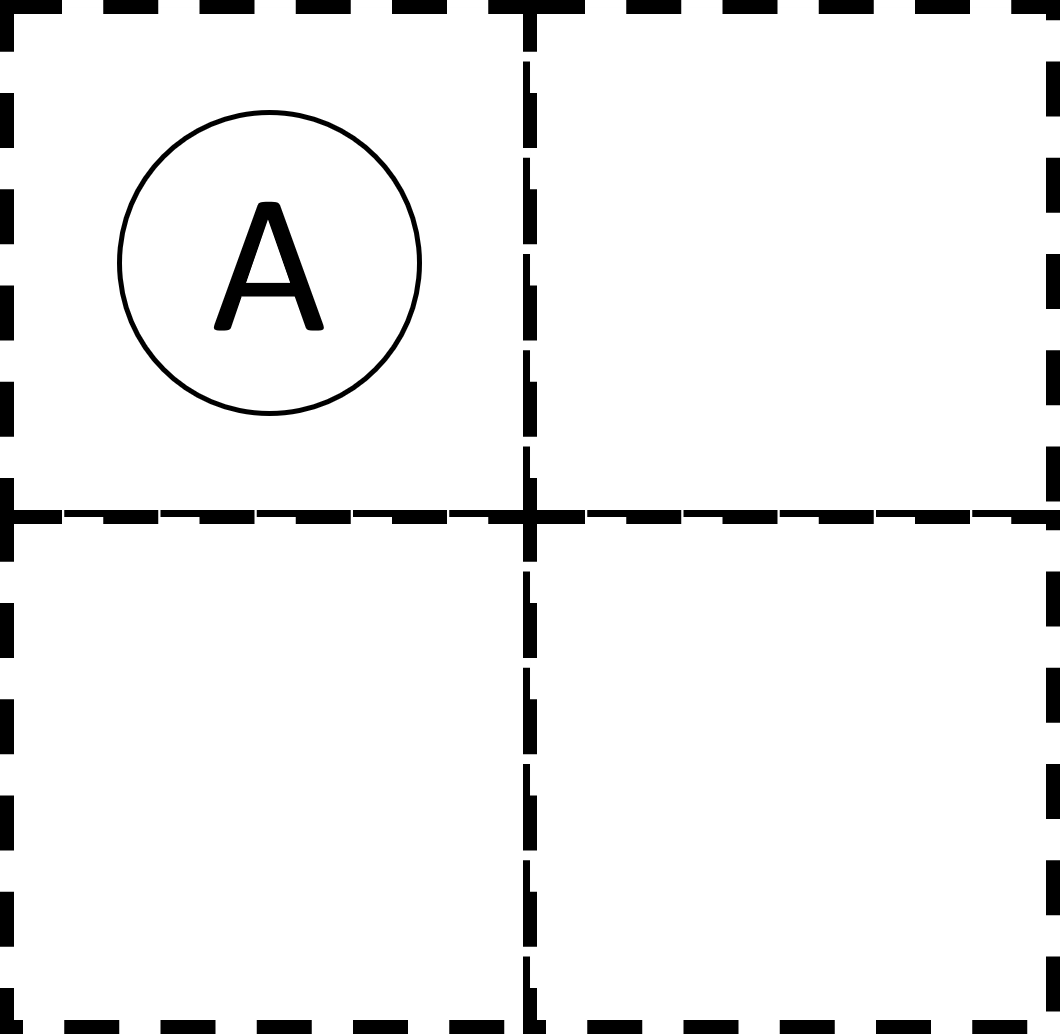
\includegraphics[width=0.5\linewidth]{2MathematicalFramework/InitialFramework/Images/2x2_no_walls_world_states/w0.png}
        \caption{$w_{0}$}
        \vspace{0.25cm}
    \end{subfigure}
    \begin{subfigure}[b]{0.45\linewidth}
        \centering
        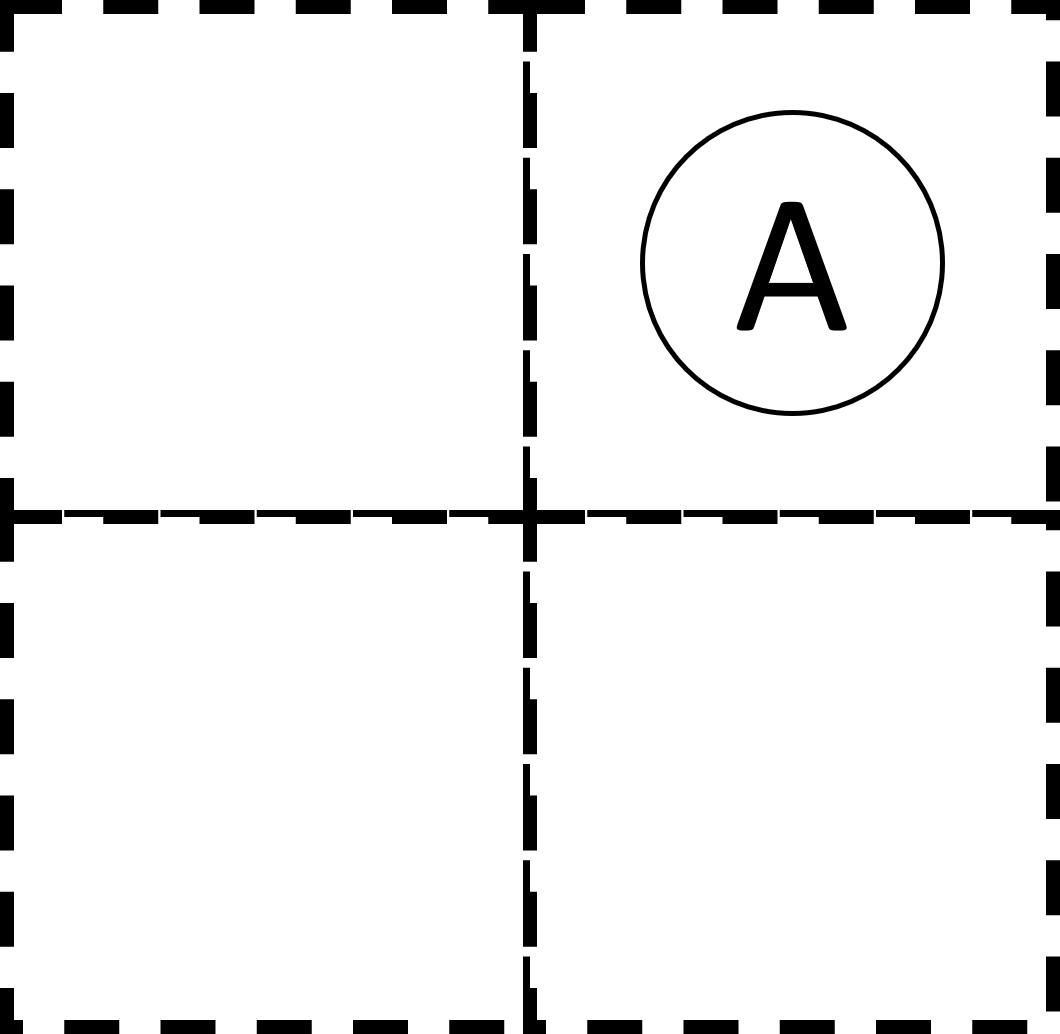
\includegraphics[width=0.5\linewidth]{2MathematicalFramework/InitialFramework/Images/2x2_no_walls_world_states/w1.png}
        \caption{$w_{1}$}
        \vspace{0.25cm}
    \end{subfigure}
    \begin{subfigure}[b]{0.45\linewidth}
        \centering
        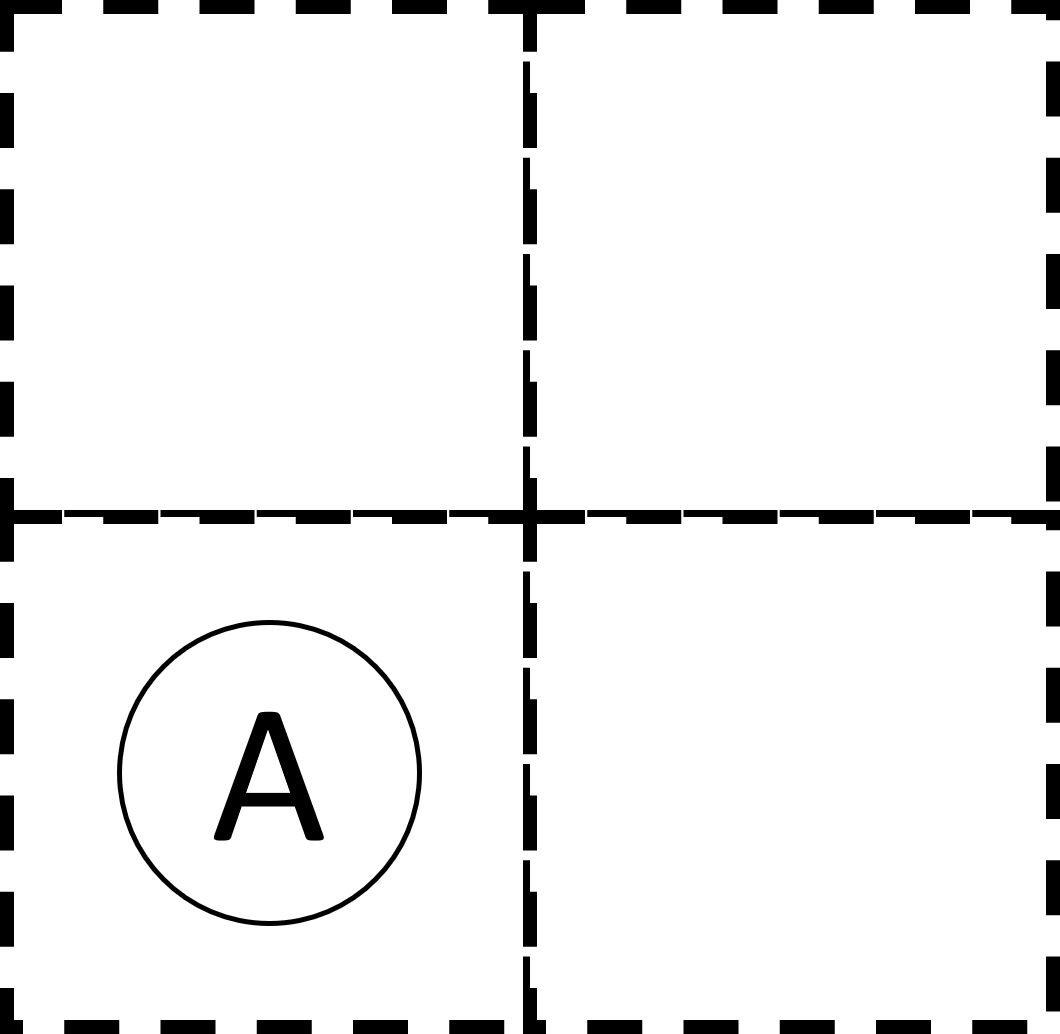
\includegraphics[width=0.5\linewidth]{2MathematicalFramework/InitialFramework/Images/2x2_no_walls_world_states/w2.png}
        \caption{$w_{2}$}
    \end{subfigure}
    \begin{subfigure}[b]{0.45\linewidth}
        \centering
        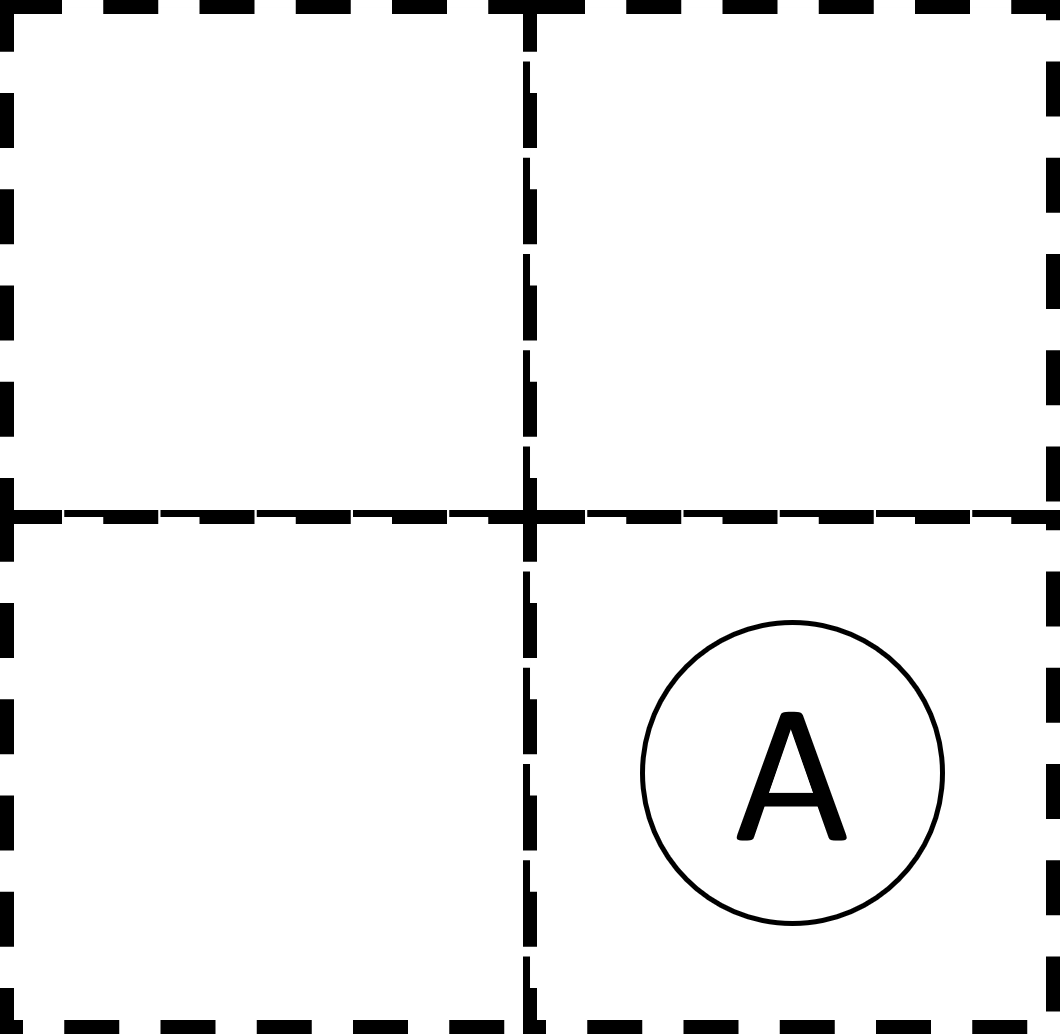
\includegraphics[width=0.5\linewidth]{2MathematicalFramework/InitialFramework/Images/2x2_no_walls_world_states/w3.png}
        \caption{$w_{3}$}
    \end{subfigure}
    \caption{The world states of a cyclical $2\times 2$ grid world $W_{c}$, where changes to the world are due to an agent moving either up, down, left, or right. The position of the agent in the world is represented by the position of the circled A.}
    \label{fig:2x2-cyclical-grid-world-states}
\end{figure}

We say the world being cyclical means that if the agent performs the same action enough times, then the agent will return to its starting position; for example, for the world $\mathscr{W}_{c}$ if the agent performs the action $U$ twice when the world is in state $w_{0}$ in Figure \ref{fig:2x2-cyclical-grid-world-states} then the world will transition into the state $w_{0}$ (i.e., $U^2 * w_{0} = w_0$).
The transition due to performing each action in each state can be found in Table \ref{tab:2x2-gridworld-minimum-transitions}.

\begin{table}
    \centering
    \begin{tabular}{c|c c c c c}
                &  $1$      & $U$       & $D$       & $L$       & $R$\\
         \hline
        $w_{0}$ & $w_{0}$   & $w_{2}$   & $w_{2}$   & $w_{1}$   & $w_{1}$\\
        $w_{1}$ & $w_{1}$   & $w_{3}$   & $w_{3}$   & $w_{0}$   & $w_{0}$\\
        $w_{2}$ & $w_{2}$   & $w_{0}$   & $w_{0}$   & $w_{3}$   & $w_{3}$\\
        $w_{3}$ & $w_{3}$   & $w_{1}$   & $w_{1}$   & $w_{2}$   & $w_{2}$\\
    \end{tabular}
    \caption{Each entry in this table shows the outcome state of the agent performing the action given in the column label when in the world state given by the row label.}
    \label{tab:2x2-gridworld-minimum-transitions}
\end{table}

The transitions shown in Table \ref{tab:2x2-gridworld-minimum-transitions} can be represented as the transition diagram given in Figure \ref{fig:2x2-cyclical-min-trans}.
It should be noted that, since the structure of the diagram is wholly dependent on the arrows between the world states, the positioning of the world states is an arbitrary choice.

\begin{figure}
    \centering
    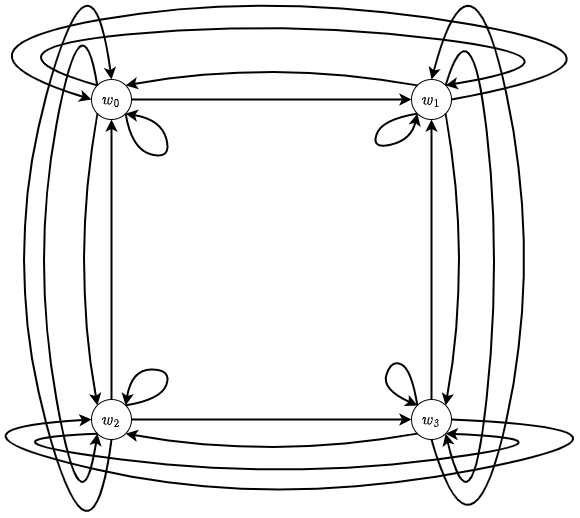
\includegraphics[width=0.5\linewidth]{2MathematicalFramework/InitialFramework/Images/2x2-cyclical-min-trans.drawio.png}
    \caption{A transition diagram for the transitions shown in Table \ref{tab:2x2-gridworld-minimum-transitions}.}
    \label{fig:2x2-cyclical-min-trans}
\end{figure}

%%%%%%%%%%%%%%%%%%%%%%%%%%%%%%%%%%%%%%%%%%%%%%%
\subsection{Agents}
We now define the actions of agents as collections of transitions that are labelled by their associated action.
We then define some relevant properties of these actions.

%%%%%%%%%%%%%%%%%%%%%%%%%%%%%%%%%%%%%%%%%%%%%%%
\textbf{Treatment of agents}
\whendraft{
\noindent\rule{\textwidth}{1mm}
\textbf{Notes:}
\begin{enumerate}
    \item Use formulation found in Higgins - agent attempts to learn the structure of the world in its representation.
\end{enumerate}
\noindent\rule{\textwidth}{1mm}
}
We now discuss how agents are treated in our model.
We consider worlds containing an embodied agent, which is able to interact with the environment by performing actions.
The end goal of the agent's learning process is to map the useful aspects of the structure of the world to the structure of its representation; the useful aspects are those that enable the agent to complete whatever task it has.

We use the treatment of agents adopted by \autocite{Higgins2018}.
The agent has an unspecified number of unspecified sensory states that allow it to make observations of the state of the environment.
Information about the world state that the agent is currently in is delivered to the internal state
\whendraft{\footnote{It is important to note that, for the purposes of this work, the agent's internal state refers to internal in the psychological sense, not in a physical sense (\textit{i.e.,} the agent's state representation not their internal organs).}} of the agent through the sensory states.
Mathematically, the process of information propagating through the sensory states is a mapping $b : W \to O$ (the `observation process'), which produces a set of observations $o_1$ containing a single observation for each sensory state.
These observations are then used by an inference process $h : O \to Z$ to produce an internal representation.
The agent then uses some internal mechanism to select an action to perform; this action is performed through active states.

The agent can be thought of as having a (non-physical) boundary between its internal state, containing its internal state representation(s) of the world, and the external world state.
Information about the world state is accessed by the internal state through sensory states only (the observation process).
The agent affects the world using active states\whendraft{\footnote{Mathematically, this is essentially a description of a single-layer Markov blanket.}}.

It is important to note that the agent's state representation only reflects the observations the agent makes with its sensors; in other words, the agent's internal state is built using the information about aspects of the world state propagated through its sensory states, in the form that the observation process provides the information, and not directly from the world state.
For example, the human eye (the sensor) converts information about the light entering the eye into electrical and chemical energy in the optic nerve (the observation process) and then the information from the optic nerve is given to the brain for inference.
Information could be lost or modified during the observation process.
For example, light sensors could only pick up certain wavelengths of light or take in a colour spectrum and output in greyscale.
This means that world states with differences that are not detectable by the agent's sensors are effectively identical from the agent's perspective and so can be treated as such when we are constructing a mathematical description of the agent's interaction with the world.

\whendraft{
[?mention Markov blanket?] [?insert explanatory diagram here?]
}


%%%%%%%%%%%%%%%%%%%%%%%%%%%%%%%%%%%%%%%%%%%%%%%
\textbf{Actions of an agent as labelled transitions}\label{sec:Agent actions as labelled transitions}
\whendraft{
\noindent\rule{\textwidth}{1mm}
\textbf{Notes:}
\begin{enumerate}
    \item $\hat{A}$ is not necessarily labelling elements of $\hat{D}$ only.
    
    \item Is $l$ actually a collection of maps $l_{w}$ for each $w \in W$ ?
\end{enumerate}
\noindent\rule{\textwidth}{1mm}
}

Consider a set $\hat{A}$ called the set of \textit{minimum actions}.
Let the set $A$ be the set of all finite \whendraft{\textbf{and infinite}} sequences formed from the elements of the set $\hat{A}$; we call $A$ the set of \textit{actions}.
Consider a set $\hat{D}_{A} \subset D$, where $1_{w} \in \hat{D}_{A}$ for all $w \in W$; we call $\hat{D}_{A}$ the set of \textit{minimum action transitions}.
We consider a labelling map $\hat{l}: \hat{D}_{A} \to \hat{A}$ such that:

\begin{enumerate}
    \item Any two distinct transitions leaving the same world state are labelled with different actions.
    \begin{action_condition}\label{actcon:action-gives-single-outcome}
        For any $d,d' \in \hat{D}_{A}$ with $s(d)=s(d')$, $\hat{l}(d) \neq \hat{l}(d')$.
    \end{action_condition}

    \item There is an identity action that leaves any world state unchanged.
    \begin{action_condition}\label{actcon:identity-action}
        There exists an action $1 \in \hat{A}$ such that $\hat{l}(1_{w})=1$ for all $w \in W$.
        We call $1$ the \textit{identity action}.
    \end{action_condition}
    
\end{enumerate}

\whendraft{
\textbf{Hidden diagram (commented out):}
% \begin{figure}
%     \centering
%     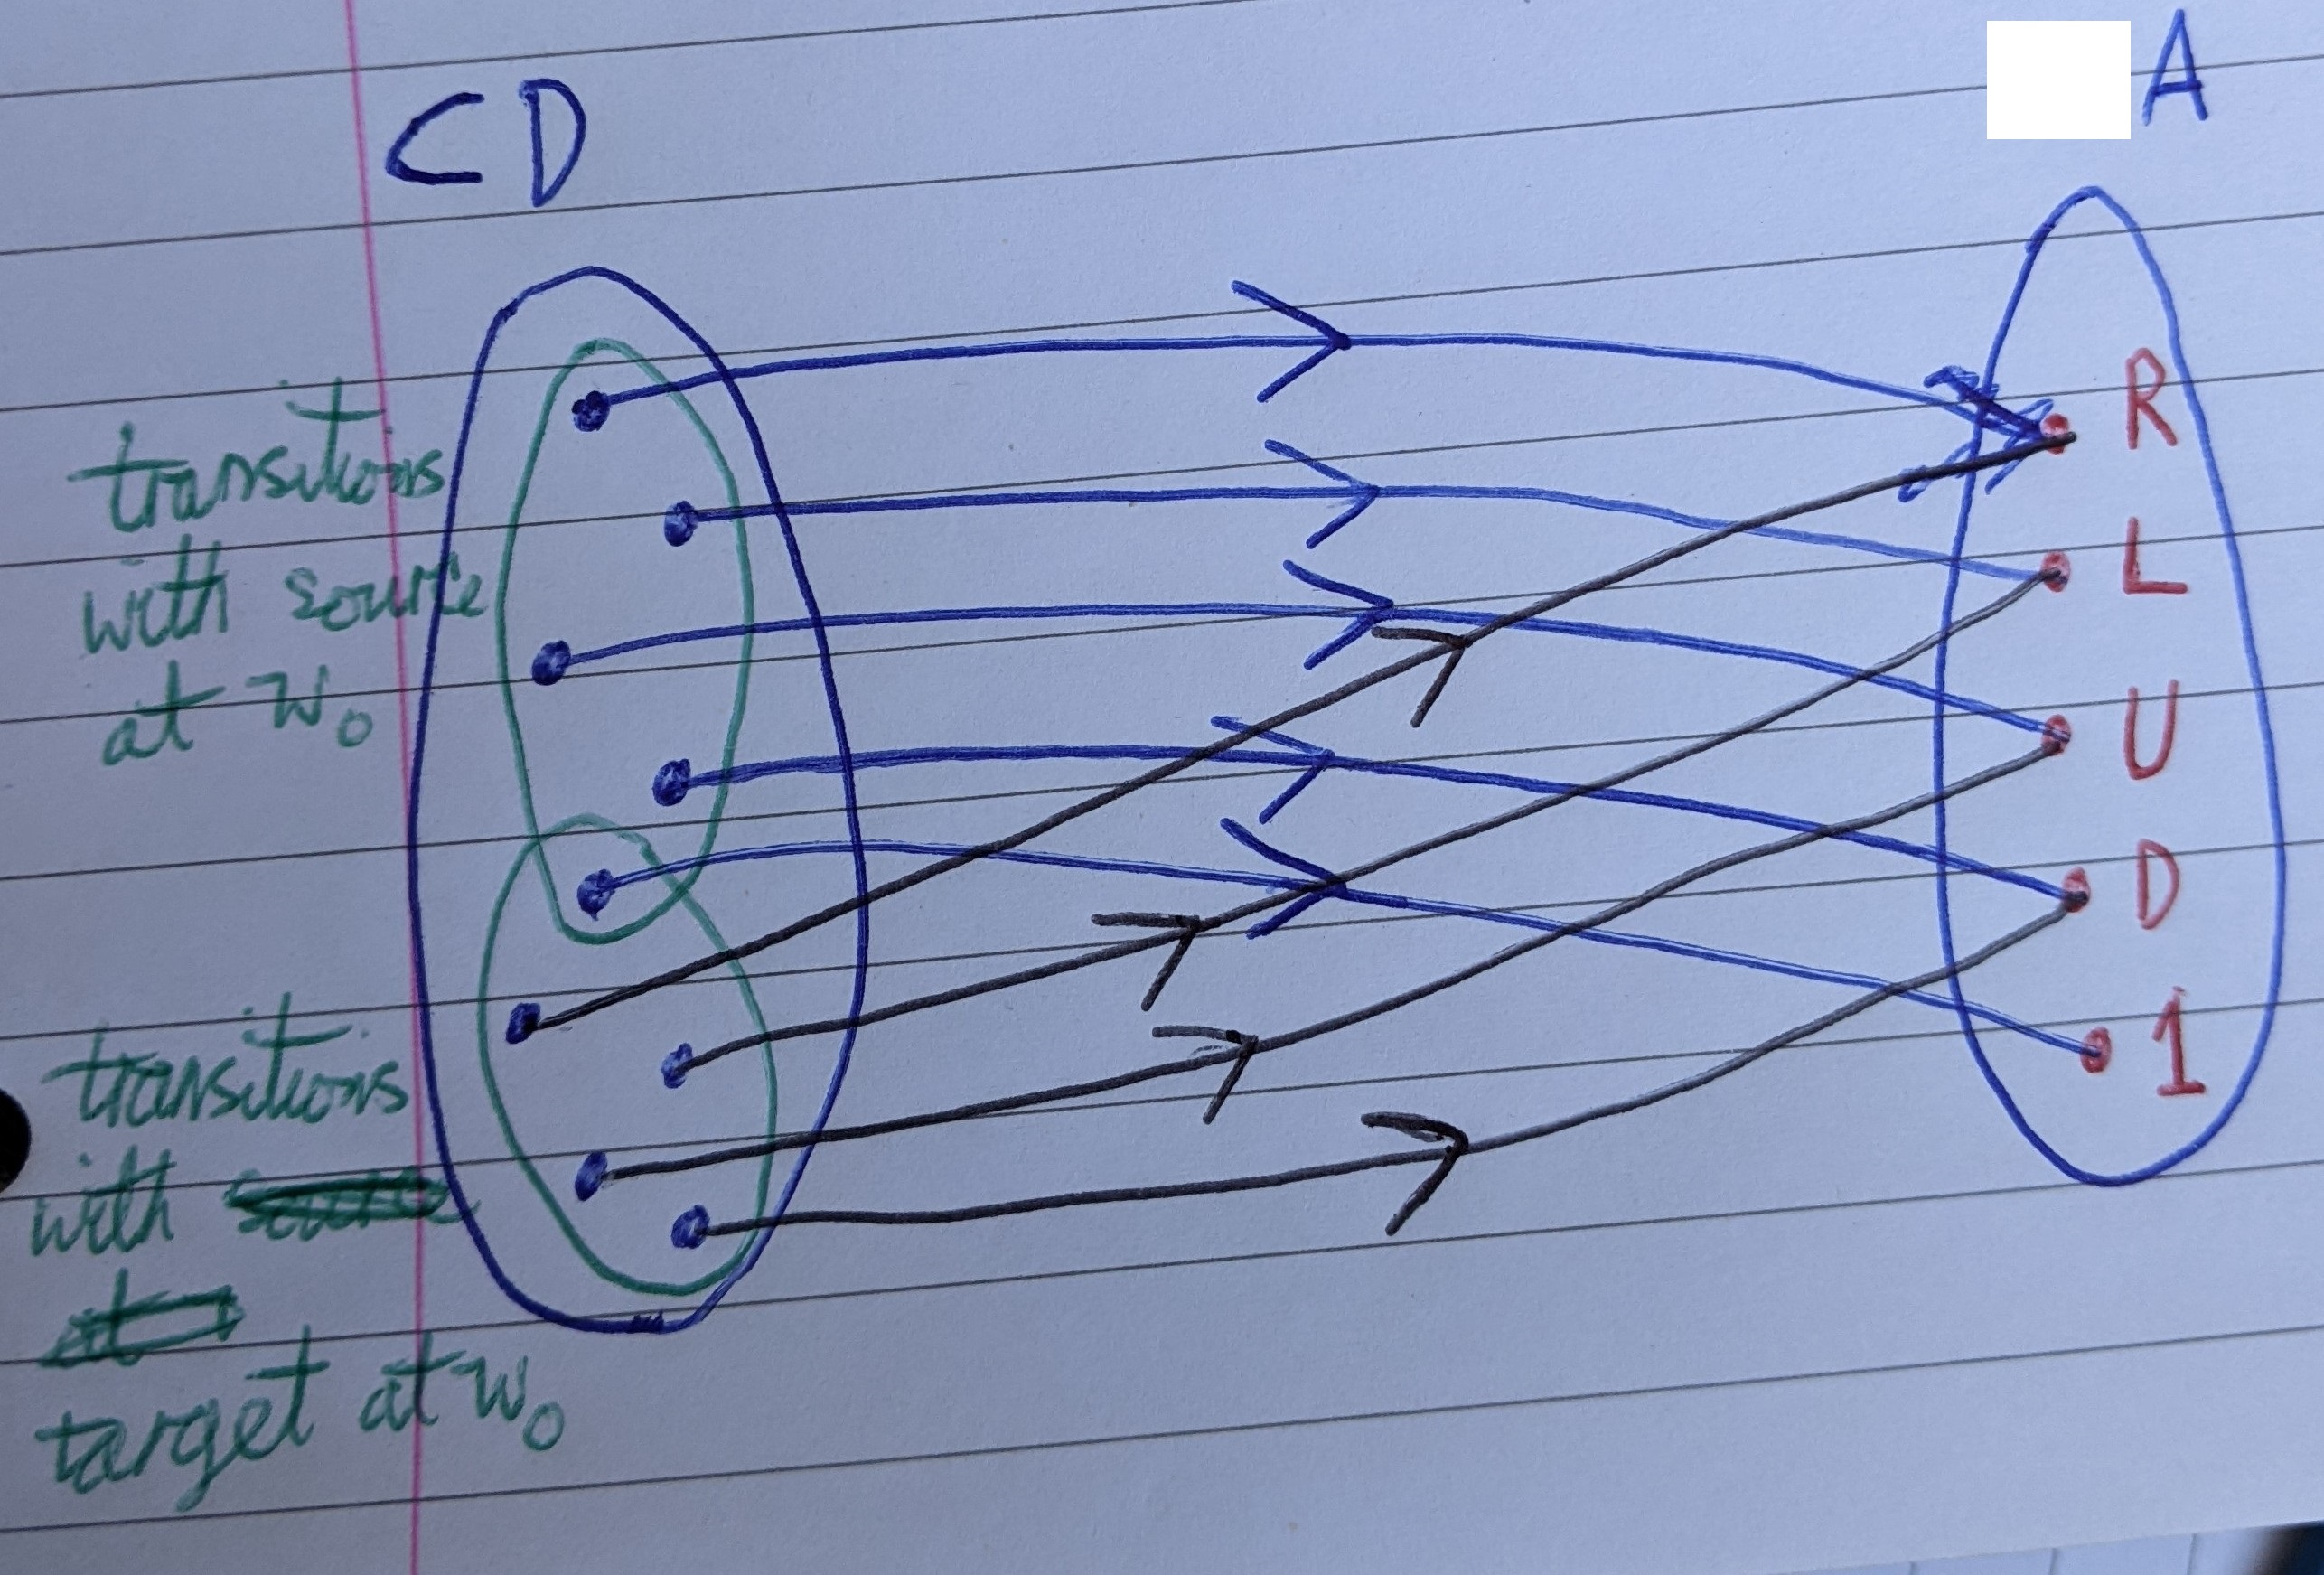
\includegraphics[width=0.5\linewidth]{Framework/Images/l-map-for-transitions-from-and-to-w0.jpg}
%     \caption{This diagram shows how the minimum transitions $d$ with $d(s) = w_{0}$ or $d(t)= w_{0}$ are mapped to actions using the map $l$.
%     }
%     \label{fig:l-map-for-transitions-from-and-to-w0}
% \end{figure}



Figure ref[fig:l-map-for-transitions-from-and-to-w0] demonstrates how the map $l$ maps transitions in $D$ to the elements in $A$ for the transitions shown in Figure \ref{fig:2x2-cyclical-min-actions-standard}.
}

\whendraft{
\begin{remark}
    \hyperref[actcon:action-gives-single-outcome]{Action condition \ref*{actcon:action-gives-single-outcome}} means that for each $w \in W$, there is a subset of $\hat{D}_{A}$ given by $\{d \mid d \in \hat{D}_{A}\textit{, } s(d)=w\}$; for each of these subsets, the elements of the subset are uniquely labelled (within the subset) by $l$.
    In other words, the transitions in $D_{A}$ with source $s(d)$ are uniquely labelled by $\hat{l}$ for all $d \in D_{A}$.
\end{remark}
}
Given $\hat{D}_{A}$ as defined above and satisfying  action condition \ref{actcon:action-gives-single-outcome} and  action condition \ref{actcon:identity-action}, we define $Q_{D_{A}} = (W, \hat{D}_{A}, s_{A}, t_{A})$, where $s_{A}, t_{A}$ are the restrictions of $s,t$ to the set $\hat{D}_{A}$.
We now define a set $D_{A}$, the set of \textit{action transitions}, which is the set of all paths of $Q_{D_{A}}$.

We extend the map $\hat{l}$ to a map $l: D_{A} \to A$ such that if $d = \hat{d}_{n} \circ ... \circ \hat{d}_{1}$ then $l(d) = \hat{l}(\hat{d}_{n}) ... \hat{l}(\hat{d}_{1})$.
For $d \in D_{A}$ with $s(d) = w$, $t(d) = w'$ and $l(d) = a$, we will often denote $d$ by $d: w \xrightarrow{a} w'$.

If an action $a \in A$ is expressed in terms of its minimum actions as $a = \hat{a}_{n} \circ ... \circ \hat{a}_{1}$, then $a = l(d) = l(\hat{d}_{n} \circ ... \circ \hat{d}_{1}) = \hat{l}(\hat{d}_{n}) \circ ... \circ \hat{l}(\hat{d}_{1}) = \hat{a}_{n} \circ ... \circ \hat{a}_{1}$, where the $\hat{a}_{i}$ are called \textit{minimum actions}.


\begin{remark}
    For a given $w \in W$, we can label transitions in $D_{A}$ with an appropriate element of $A$ through the following: for each $d \in D_{A}$ with $s(d)=w$, express $d$ in terms of its minimum transitions in $D_{A}$ as $d = d_{n} \circ ... \circ d_{2} \circ d_{1}$; if $\hat{l}(d_{i}) = a_{i}$ then $d$ is labelled with $a_{n}...a_{2}a_{1} \in A$.
    We denote the map that performs this labelling by $l: D_{A} \to A$.
\end{remark}

Figure \ref{fig:2x2-cyclical-min-actions-standard} shows how transitions are labelled with actions in our $2 \times 2$ cyclical world example.
We only show the minimum actions for simplicity but there are actually infinite action transitions between each pair of world states; for example, the action transitions from $w_{0}$ to $w_{1}$ include those labelled by: $D \circ R$, $D \circ R \circ 1^{n}$ ($n \in \mathbb{N}$), $1^{n} \circ D \circ R$ ($n \in \mathbb{N}$), $D \circ R \circ (L \circ R)^{n}$ ($n \in \mathbb{N}$) etc...

\begin{figure}
    \centering
    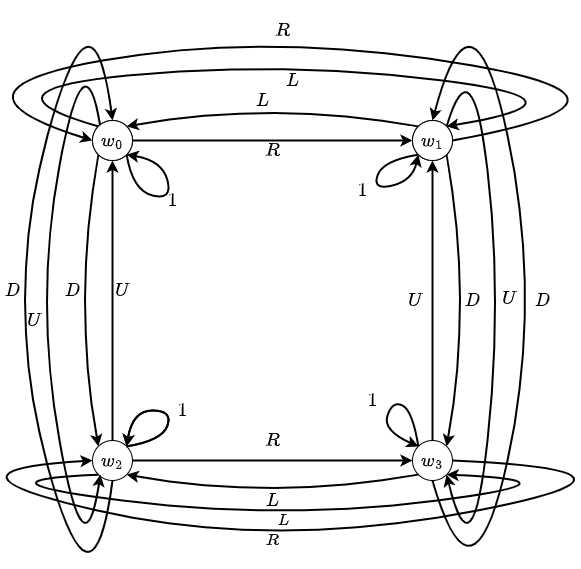
\includegraphics[width=0.5\linewidth]{2MathematicalFramework/InitialFramework/Images/2x2-cyclical-min-actions.drawio.png}
    \caption{Labelling the transitions in Figure \ref{fig:2x2-cyclical-min-trans} with the relevant actions in $A$.}
    \label{fig:2x2-cyclical-min-actions-standard}
\end{figure}

\paragraph{Effect of actions on world states}
We define the effect of the action $a \in A$ on world state $w \in W$ as the following: if there exists $d \in D_{A}$ such that $s(d)=w$ and $l(d)=a$, then $a * w = t(d)$; if there does not exist $d \in D_{A}$ such that $s(d)=w$ and $l(d)=a$, then we say that $a * w$ is \textit{undefined}.
The effect of actions on world states is well-defined due to action condition \ref{actcon:action-gives-single-outcome}.
We can apply the minimum actions that make up an action to world states individually: if $a * w$ is defined and $a = \hat{a}_{k}...\hat{a}_{1}$ then $a * w = (\hat{a}_{k}...\hat{a}_{1}) * w = \hat{a}_{k}...\hat{a}_{2} * (\hat{a}_{1} * w)$.
Physically, the identity action $1 \in A$ corresponds to the no-op action (\textit{i.e.}, the world state does not change due to this action).

\paragraph{Actions as (partial) functions}
Consider all the transitions that are labelled by a particular action $a \in A$.
Together these transitions form a partial function $f_{a}: W \to W$ because for any $w \in W$ either $a * w$ is undefined or $a * w$ is defined and there is a unique world state $w' \in W$ for which $a * w = w'$ (due to condition 1).
$f_{a}$ is not generally surjective because for a given $w \in W$ there is not necessarily a transition $d \in D$ with $l(d) = a$ and $t(d) = w$.
$f_{a}$ is not generally injective because it is possible to have an environment where $f_{a}(w)=f_{a}(w')$ for some $w \in W$ different from $w' \in W$.
We can also reproduce these functions using the formalism given by \autocite{caselles2019symmetry}, which describes the dynamics of the world in terms of a multivariate function $f: A \times W \to W$.
If we let $f: A \times W \to W$ be the dynamics of the environment then the transition caused by an action $a \in A$ on a world state $w \in W$ (where $a * w$ is defined) is given by $(a,w) \mapsto f(a,w) = a * w$.
Mathematically, we curry the function $f: A \times W \to W$ to give a collection $\{f_{a}\}$ of partial functions with a partial function $\hat{f}(a)=f_{a}: W \to W$ for each action $a \in A$ as $\textit{Curry}: (f: A \times W \to W) \to (f_{a}: W \to W)$.
